\subsection{Coloración de vértices de un grafo}

\begin{prob}
    Suponga que queremos organizar 6 eventos de una hora en una convención, estos eventos son $v_1, v_2, v_3, v_4, v_5, v_6$, y entre la audiencia hay gente que quiere ir al mismo tiempo a:
    
    \break
    \begin{itemize}
        \item $v_1$ y $v_2$.
        \item $v_1$ y $v_4$.
        \item $v_3$ y $v_5$.
        \item $v_2$ y $v_6$.
        \item $v_4$ y $v_5$.
        \item $v_5$ y $v_6$.
        \item $v_1$ y $v_6$.
    \end{itemize}
    
    ¿Cuántas horas harán falta para que los eventos puedan darse sin chocar entre la audiencia?
    \end{prob}
    
    \begin{proof}[Solución]
    La situación general se puede representar mediante el siguiente grafo:
    
    \begin{figure}
    \centering
    \begin{tikzpicture}
        \GraphInit[vstyle=Welsh]
        \Vertices[unit=2]{circle}{$v_3$, $v_2$, $v_1$, $v_6$, $v_5$, $v_4$}
        \Edges($v_1$,$v_2$,$v_6$,$v_1$,$v_4$,$v_5$,$v_6$,$v_5$,$v_3$)
    \end{tikzpicture}
    \caption{Cada vértice de este grafo representa un evento, y cada lado un potencial choque.}
    \label{fig:nocolor}
    \end{figure}
    
    \noindent donde los vértices representan los eventos y los lados representan los potenciales choques. El problema se resuelve al tomar los pares de vértices que \textbf{no} están conectados. Luego, una solución puede ser la siguiente:
    
    \begin{center}
        \begin{tabular}{cccc}
            \text{Hora 1} & \text{Hora 2} & \text{Hora 3} & \text{Hora 4} \\ \toprule
            $v_1$ \text{ y } $v_3$ & $v_2$ \text{ y } $v_4$ & $v_5$ & $v_6$
        \end{tabular}
    \end{center}
\end{proof}

En términos matemáticos, lo que hemos hecho es asignar una partición de cuatro partes al conjunto de vértices del grafo, con la condición de que ninguna de dichas partes contenga un par de vértices adyacentes.

A estas partes les llamamos \textbf{colores} en lugar de horas, pero la naturaleza exacta de los objetos no es importante.

\begin{defn}
    Sea $G=(V,L)$ un grafo. Una \ul{$r$-coloración} de $V$ es una función $f: V \rightarrow \{ 1, 2, \dots, r \}$ con $r \in \Nastk$ tal que $xy \in L \implies f(x) \neq f(y)$.
    
    La idea de este concepto será encontrar el mínimo $r$ tal que existe una $r$-coloración de los vértices de un grafo. Este es el \ul{número cromático}, y se representa con $\chi(G)$.
\end{defn}

De esta forma, si decidimos asignar un color a cada uno de los vértices del grafo \ref{fig:nocolor}, nos queda

\begin{figure}
    \centering
    \begin{tikzpicture}
        \GraphInit[vstyle=Welsh]
        \Vertices[unit=2]{circle}{$v_3$, $v_2$, $v_1$, $v_6$, $v_5$, $v_4$}
        \Edges($v_1$,$v_2$,$v_6$,$v_1$,$v_4$,$v_5$,$v_6$,$v_5$,$v_3$)
        \SetVertexNoLabel
        \AddVertexColor{red}{$v_1$,$v_3$}
        \AddVertexColor{blue}{$v_2$, $v_4$}
        \AddVertexColor{green}{$v_5$}
        \AddVertexColor{yellow}{$v_6$}
    \end{tikzpicture}
    \caption{El mismo grafo con la coloración planteada en la tabla.}
    \label{fig:color}
\end{figure}

\noindent sin embargo, este no es el menor número de colores que se pueden usar. Como los vértices $v_1$, $v_2$ y $v_6$ forman un triángulo, es decir, un grafo $K_3$, cada uno de ellos necesita un color distinto por ser adyacente a los otros dos, por lo que se necesitan al menos 3 colores para pintar el grafo completo.

\begin{figure}
    \centering
    \begin{tikzpicture}
        \GraphInit[vstyle=Welsh]
        \Vertices[unit=2]{circle}{$v_3$, $v_2$, $v_1$, $v_6$, $v_5$, $v_4$}
        \Edges($v_1$,$v_2$,$v_6$,$v_1$,$v_4$,$v_5$,$v_6$,$v_5$,$v_3$)
        \SetVertexNoLabel
        \AddVertexColor{red}{$v_1$}
        \AddVertexColor{blue}{$v_2$, $v_5$}
        \AddVertexColor{green}{$v_3$, $v_4$, $v_6$}
    \end{tikzpicture}
    \caption{Nuevamente el mismo grafo, pero utilizando menos colores.}
    \label{fig:color2}
\end{figure}

\begin{prob}
    ¿Cuál es el número cromático de un grafo cíclico $C_{2r}$ con un número par de vértices, y de uno $C_{2r+1}$ con un número impar de vértices?
\end{prob}

\begin{proof}[Solución]
    En el caso de los grafos cíclicos, si tenemos un ciclo par con una cantidad par de vértices, los vértices que tengan índice par tendrán un color distinto a los vecinos que tengan índice impar, pero como estos vértices se van turnando, con dos colores es suficiente para pintar el grafo. Si tenemos una cantidad impar de vértices, necesitaremos dos colores, y con ellos será suficiente para pintar $2r$ vértices, pero al agregar el vértice que falta, tendremos que este es vecino de un vértice con índice par, y de otro con vértice impar, por lo que necesitaremos un color adicional para pintar este último vértice, dándonos en total tres colores distintos.
\end{proof}

\begin{defn}
    Un grafo se dice que es \ul{bipartito} si se puede hallar una 2-partición de sus vértices tal que los vecinos de una están en la otra.
    
    Se tiene que, por definición
    
    \[
    \chi(G) = 2 \iff \text{$G$ es bipartito}
    \]
\end{defn}

Luego, si $G$ contiene un ciclo impar, entonces $\chi(G) \geq 3$. Por lo que podemos también decir que 

\[
\text{$G$ es bipartito} \implies \text{no hay ciclos impares en $G$}
\]

\begin{pre}
    ¿Si $G$ no tiene ciclos impares, entonces $\chi(G) = 2$?
\end{pre}
    
\begin{proof}[Respuesta]
    Sin pérdida de generalidad, supongamos que $G$ es conexo. Escojamos cualquier vértice y llamemoslo $v_1$ y diremos que está en el \textit{nivel 0}. Tomemos $v_2, \dots, v_r$, los vecinos de $v_1$ y diremos que están en el \textit{nivel 2}. Procediendo de esta forma, en el \textit{nivel $k$} habremos asignado todos los vértices adyacentes a los vértices del \textit{nivel $k-1$}, pero no aquellos del \textit{nivel $k-2$}.
    
    Al ordenar los vértices de esta forma, tendremos que los vértices en el \textit{nivel $k$} son adyacentes únicamente a los vértices del \textit{nivel $k-1$} y el \textit{nivel $k+1$}, y no a los del mismo nivel. Esto indica que, si tomamos dos vértices $x$ e $y$ en el mismo nivel, estos están unidos por un camino $m$ de igual longitud a cualquier vértice $z$ ubicado en algún nivel anterior, y los caminos se pueden elegir de forma tal que $z$ es el único vértice en común.
    
    Si $x$ e $y$ fuesen adyacentes, tendríamos que hay un ciclo de longitud impar $2m+1$, contrario a la hipótesis. Por lo tanto, si asignamos un color a los vértices de niveles pares, y otro a los vértices de niveles impares, tenemos $\chi(G)=2$.
    
    Y de esta forma, queda resuelto. La respuesta es afirmativa.
\end{proof}

Así, ya tenemos la demostración del teorema que enunciaremos a continuación.

\begin{teo}
    Un grafo es bipartito si y sólo si no contiene ciclos de longitud impar.
\end{teo}

\subsection{El algoritmo voraz}

Conseguir el número cromático de un grafo dado es un problema difícil. Sin embargo, si existe un método con el que construir una coloración de vértices utilizando una cantidad razonable de colores.

Este método consiste en asignar colores a los vértices en orden, de tal forma que cada vértice recibe el primer color que no haya sido asignado a uno de sus vecinos. En este algoritmo tomaremos la mejor desición que podamos en cada paso, sin tomar en cuenta si esta elección traerá problemas más adelante. Un algoritmo de este estilo se conoce como \textbf{algoritmo voraz}.

\begin{teo}
    Si $G$ es un grafo con máximo grado $k$, entonces
    
    \begin{enumerate}
        \item $\chi(G) \leq k+1$.
        \item Si $G$ es conexo y no regular, $\chi(G) \leq k$.
    \end{enumerate}
\end{teo}

\begin{proof}
    Pasemos a demostrar cada punto en orden:
    
    \begin{enumerate}
        \item Sean $v_1, \dots, v_n$ los vértices del grafo $G$. Entonces, para cualquiera de estos vértices, este tiene a lo sumo $k$ vecinos, por lo que el algoritmo voraz puede asignar a lo sumo $k$ colores a los vecinos de $v_i$. Por lo tanto, a $v_i$ se le asignará un color distinto. Y es en este sentido donde tenemos $k+1$ colores, por lo tanto $\chi(G) \leq k+1$.
        \item Como $G$ tiene grado máximo $k$ y no es regular entonces habrá al menos un vértice $v_n$ con grado menor a $k$. Entonces, tomemos en cuenta todos los vértices $v_{n-1}, v_{n-2}, \dots, v_{n-r}$ vecinos de $v_n$; hay a lo sumo $k-1$. Ahora, si consideramos los vecinos de $v_{n-1}$, tendremos a lo sumo $k-1$. Procediendo de manera sucesiva (y sin considerar los vértices que ya han sido considerados anteriormente), llegará un punto en el que consideraremos a todos los vértices del grafo $G$, ya que este está conectado. Como para cada uno de estos vértices se tienen a lo sumo $k-1$ vecinos, entonces procediendo con el algoritmo voraz tendremos a lo sumo $k-1$ colores para asignarle a cada uno. Si además contamos el color del vértice que estamos considerando, tendremos en total $k$ colores. Es en este sentido que tendremos $\chi(G) \leq k$.
    \end{enumerate}
    
    De esta forma, queda demostrado el teorema.
\end{proof}